%----------------------------------------------------------------------------
\chapter{Feladatspecifikáció}
\label{sec:Sepcification}
%----------------------------------------------------------------------------

Ebben a fejezetben bemutatom az alkalamzás céljait. Az első részben általános összefoglalom a felhasználói elvárásokat és legfőbb építőköveket a programzó szemszögéből.
Ezt követően megmutatom a használati Usecaseeket.

Kitérek a főbb funkciókra, azok felépítésére és elvárt használati módjaira.
Az utolsó fejezetben mindezt egy Usecase UML diagramban összefoglalom.
Megtalálható benne az összes fent leírt használati eset, jól látható lesz, hogy a funkciók hasonlítanak egymásra így a felhasználó könnyen meg tudja tanulni az alkalmazás használatát.

\section{Feladat részletes leírása}
\label{sec:SepcificationDescription}

Ebben az alszakaszban részletesen kitérek az alkalamazás komponenseinek megtervezésére, és azok használatára.
Bemutatom, hogy milyen egy feladatsor felépítése, és annak a részei milyen mezőket vagy értékeket tartalmaznak.
Ebben a részben szövegesen végig éehet kísérni a \ref{fig:UsecaseDiagram}.~ábrán látható felépítést.

\subsection{Általános célok bemutatása}


A program célja az, hogy egy vagy több felhasználó létre tudjon hozni igaz-hamis illetve feleletválasztós (tetszőleges számú válaszopcióval) kérdésekből álló feladatsort.
Az alaklamazás csak papír alapú kitöltést támogat, ezt olyan formában teszi, hogy az összeállító a kész kérdéssort ki tudja exportálni PDF formátumba.

A szoftver a fent leírtakon kívül rendelkezik egy automtizált javítási rendszerrel, okostelefont használva a Google ML Kit\cite{MLKit} segítségével be lehet scannelni egy megfelelően formázott választ, és az belekerül egy form-ba amit a szervernek elküldve visszaküldi az eredményt.
A kézírásos szövegfelismerés sok esetben nem szolgáltatott megfelelően pontos eredményt, így ez a funkció csak alpha verzióban támogatott.
Hibásan felismert, vagy felismerhetetlen váaszok esetén kézzel is szerkeszthető a válasz a kiértékelés előtt.

Az alkalmazás a főmenüből indul, innen lehet tovább navigálni az összes opcióhoz.
A főmenü máshogy néz ki a használt eszköztől függően.
A választásunk után egy listázó nézet tárul elénk, ahol látjuk az adott opcióhoz tartozó összes eddig felvett elemet.
Itt tudunk új elemet is hozzáadni az adott kategórihoz, illetve a listán történő kattintással a részletes nézet tárul elénk.
A részletes nézeten minden adatot egyszerre látunk, itt tudjuk törölni és módosítani is.
Mind a létrehozás és a szerkesztés során *-gal vannak jelölve a kötelező értékek. Törlés során van egy figyelemfelhívó ablak is, mivel a törlés az végleges és nem vonható vissza.
Vannak egyediséget megkívánó mezők, így amennyiben már létezik a megadott értékkel egy felvett elem, jelzi a za alkalmazás, hogy ezt módosítani kell mentés előtt.

A szoftver müködési elve és kommunikációja röviden összefoglalva az alábbi.
A felhasználó megnyitja az alkalamzást, majd interaktál akezelő felülettel.
A kattintások során amik igénylik az adatbázis elérést (listázás, részletes nézet megjelenítése, új elem létrehozása, szerkesztés, törlés) az alaklamazás szabványos HTTP kéréseket intéz a REST API-hoz.
Az adatok forgalma szabványos JSON formátummal zajlik mind az adatküldés, mind az adatok fogadása során mindkét irányban.
A REST API és az adatbázis is egy virtuális gépen fut egy-egy Docker konténerben.


\subsection{Egy feladatsor felépítése}

Egy feladatsor a következő elemekből épül fel:

\begin{itemize}
	\item \emph{Témakör}
	\item \emph{Kérdések:}
        \begin{itemize}
            \item \emph{Igaz-hamis:} A szokásos egyszerű igaz-hamis típusfeladat.
                \begin{itemize}
                    \item \emph{Kérdés:} Meg kell adni magát az eldöntendő kérdést.
                    \item \emph{Pontozási módszer:} Egyedi pontozási módszert lehet létrehozni. Beállítható az összpontszám és a helyes és helytelen válaszokra adott pontérték, amely lehet negatív is.
                    \item \emph{Témakör:} Segít a kérdések kategorizálásában és szűrésében az összeállítás során.
                    \item \emph{Helyes válasz:} Szükséges a javítás elvégzéséhez.
                \end{itemize}
            \item \emph{Feleletválasztós:} A szokásos egyszerű feleletválasztós típusfeladat, testreszabható mennyiségű válaszopcióval.
                \begin{itemize}
                    \item \emph{Kérdés:} Meg kell adni magát a kérdést, több helyes válasz is lehetséges.
                    \item \emph{Pontozási módszer:} Egyedi pontozási módszert lehet létrehozni. Beállítható az összpontszám és a helyes és helytelen válaszokra adott pontérték, amely lehet negatív is.
                    \item \emph{Témakör:} Segít a kérdések kategorizálásában és szűrésében az összeállítás során.
                    \item \emph{Válaszok:} Meg kell adni a válaszopciókat.
                    \item \emph{Helyes válasz(ok listája):} Szükséges a javítás elvégzéséhez.
                \end{itemize}
        \end{itemize}
\end{itemize}

\subsection{Komponensek létrehozásának lépései}

Az alábbiakban bemutatom az egyes alkotóelemek életútját az alkalmazáson belül.

\subsubsection{Pont}

A pontok listáját az ennek megfelelő menüpont kiválasztása után érjük el.
Itt egy floating button segítségével adhatunk új pontot az alkalmazáshoz.
A létrehozáshoz, amelyet szintén egy floating button segítségével érhetünk el a részletes nézetről, minden mező kitöltése kötelező, csak így biztosítható megfelelően az elvárt működése a javítási funkció miatt.

\begin{itemize}
    \item \emph{Típus/Név:} A pont típusa vagy neve. Ez egyedi mező is egyben, így lehet rá hivatkozni és megtalálni az alkalmazásban.
    \item \emph{Pont:} A feladatra adható maximális pontszám.
    \item \emph{Helyes válasz:} A helyes válaszokra adható pont, ajánlott úgy megvalósítani a pontozást, hogy ezeknek az összege a teljes pontszám legyen.
    \item \emph{Helytelen válasz:} A helytelen válaszok során levont pontmennyiség. Amennyiben nincs levonás, az értéke 0; egyébként egy negatív szám.
\end{itemize}

A pont létrehozása után látható lesz a listás nézetben, ahol kiválasztva ellenőrizhetjük a megadott értékeket, szükség esetén módosíthatjuk is.
A pontokat törölni is lehet, de csak akkor, ha egyetlen kérdéshez sem használjuk, különben inkonzisztens állapot alakulna ki és pont nélküli kérdések keletkeznének.
Mindkét műveletet a részletes oldalon tehetjük meg.

\subsubsection{Témakör}

A témák listáját az ennek megfelelő menüpont kiválasztása után érjük el.
Itt egy floating button segítségével adhatunk új témakört az alkalmazáshoz.
A létrehozáshoz, amelyet szintén egy floating button segítségével érhetünk el a részletes nézetről, minden mező kitöltése kötelező, csak így biztosítható megfelelően az elvárt működés.

\begin{itemize}
    \item \emph{Témakör neve:} A témakör megnevezése, egyedi mező.
    \item \emph{Témakör leírása:} Kötelező egy rövid leírást adni az egyértelműség érdekében.
    \item \emph{Szülő témakör:} Megadható egy fölérendelt témakör is.
\end{itemize}

A témakör létrehozása után látható lesz a listás nézetben, ahol kiválasztva ellenőrizhetjük a megadott értékeket, szükség esetén módosíthatjuk is.
A témaköröket törölni is lehet, de csak akkor, ha egyetlen kérdéshez és feladatsorhoz sem használjuk, különben inkonzisztens állapot alakulna ki, és témakör nélküli kérdések és feladatsorok keletkeznének.
Mindkét műveletet a részletes oldalon tehetjük meg.

\subsubsection{Igaz-hamis kérdés}

Az igaz-hamis kérdések listáját az ennek megfelelő menüpont kiválasztása után érjük el.
Itt egy floating button segítségével adhatunk új kérdést az alkalmazáshoz.
A létrehozáshoz, amelyet szintén egy floating button segítségével érhetünk el a részletes nézetről, minden mező kitöltése kötelező, csak így biztosítható megfelelően az elvárt működés.

\begin{itemize}
    \item \emph{Témakör neve:} A kérdéshez tartozó témakör megnevezése, a meglévő elemek közül választható.
    \item \emph{Pont típusa:} A kérdéshez tartozó pont megnevezése, a meglévő elemek közül választható.
    \item \emph{Kérdés:} A kérdés szövege, egyedinek kell lennie.
    \item \emph{Helyes válasz:} Meg kell adni a helyes válaszopciót, amely lehet igaz vagy hamis.
\end{itemize}

A kérdés létrehozása után látható lesz a listás nézetben, ahol kiválasztva ellenőrizhetjük a megadott értékeket, szükség esetén módosíthatjuk is.
A kérdéseket törölni is lehet, de csak akkor, ha egyetlen feladatsorhoz sem használjuk, különben inkonzisztens állapot alakulna ki, és hiányoznának kérdések az összeállított feladatsorokból.
Mindkét műveletet a részletes oldalon tehetjük meg.

\subsubsection{Feleletválasztós kérdés}

A feleletválasztós kérdések listáját az ennek megfelelő menüpont kiválasztása után érjük el.
Itt egy floating button segítségével adhatunk új kérdést az alkalmazáshoz.
A létrehozáshoz, amelyet szintén egy floating button segítségével érhetünk el a részletes nézetről, minden mező kitöltése kötelező, csak így biztosítható megfelelően az elvárt működés.

\begin{itemize}
    \item \emph{Témakör neve:} A kérdéshez tartozó témakör megnevezése, a meglévő elemek közül választható.
    \item \emph{Pont típusa:} A kérdéshez tartozó pont megnevezése, a meglévő elemek közül választható.
    \item \emph{Kérdés:} A kérdés szövege, egyedinek kell lennie.
    \item \emph{Válaszok megadása:} Meg kell adni a válaszokat, és jelölni kell a helyes válaszokat.
\end{itemize}

A kérdés létrehozása után látható lesz a listás nézetben, ahol kiválasztva ellenőrizhetjük a megadott értékeket, szükség esetén módosíthatjuk is.
A kérdéseket törölni is lehet, de csak akkor, ha egyetlen feladatsorhoz sem használjuk, különben inkonzisztens állapot alakulna ki, és hiányoznának kérdések az összeállított feladatsorokból.
Mindkét műveletet a részletes oldalon tehetjük meg.

\subsubsection{Feladatsor}
\label{sec:SpecificationExamDescription}

A feladatsorok listáját az ennek megfelelő menüpont kiválasztása után érjük el.
Itt egy floating button segítségével adhatunk új feladatsort az alkalmazáshoz.
A létrehozáshoz, amelyet szintén egy floating button segítségével érhetünk el a részletes nézetről, minden mező kitöltése kötelező, csak így biztosítható megfelelően az elvárt működés.

\begin{itemize}
    \item \emph{Feladatsor neve:} Egyedi mező.
    \item \emph{Témakör kiválasztása:} A kérdéshez tartozó témakör megnevezése, a meglévő elemek közül választható.
\end{itemize}

A feladatsor létrehozása után látható lesz a listás nézetben, ahol kiválasztva a részletes oldalt látjuk.
Itt van lehetőségünk a kérdések hozzáadására és eltávolítására a feladatsorból.
A témákra és kérdéstípusokra szűrve válogathatunk a kérdéseink között.
Hozzáadás után a kérdések mozgathatóak a listában.
A más típusuba tartozó kérdések más színnel vannak jelölve ezzel is segítve a felhasználót a kérdés típusának gyors felmérésében.
A feladatsorok szabadon törölhetők.
Innen léphetünk át a szerkesztés oldalra, ahol a nevet és a témakört tudjuk módosítani.

\subsubsection{Válaszok ellenőrzése}

Amennyiben ezt a menüpontot választjuk, akkor a \refstruc{sec:SpecificationExamDescription}-ban is leírt feladatsor listát látjuk, innen is létre lehet hozni új feladatsort.
Az itt kiválasztott elem viszont egy form beküldő oldalra navigál, ahol egymás alatt látszanak a kérdések.
A más típusuba tartozó kérdések más színnel vannak jelölve ezzel is segítve a felhasználót a kérdés típusának gyors felmérésében.

Itt lehet megadni a válaszainkat, illetve mobil eszközön a szövegfelismerés funkciója gyorsíthatja meg a kitöltést.
A lehetséges formátumra, amit a szoftver elvár található segítség, így nehezebb ezért rossz megoldást megadni.
Ha mégis hibás formátumban küldi be a felhasználó a válaszokat kap róla figyelmeztetést.
A beküldést követően hamarosan megjelenik az eredmény a képernyőn.

\subsubsection{Feladatsorok exportálása}

Amennyiben ezt a menüpontot választjuk, akkor a \refstruc{sec:SpecificationExamDescription}-ban is leírt feladatsor listát látjuk, innen is létre lehet hozni új feladatsort.
Az itt kiválasztott elem viszont egy előzetes feladatsor megjelenítő oldalra navigál.

Amennyiben az itt látottakkal elégedettek vagyunk, rendben vannak a pontok és a kérdések, akkor exportálhatjuk is a munkát PDF formátumban.
Az itt látottak csak egy vázlatos elrendezést adnak; az adatok ellenőrzésére szolgálnak.
Előfordulhat, hogy a mobilos és az asztali verzió kis mértékben eltér egymástól a megjelenésben.

\section{Diagramok}
\label{sec:SpecificationDiagrams}

Ebben az alfejezetben az elkészült alkalmazás használati eseteit bemutató diagram található.  
A használati eseteket ábrázoló diagram (use case diagram) segítségével egy tapasztalt fejlesztő gyorsan fel tudja mérni az alkalmazás fő felépítését, funkcióit és megközelítő struktúráját.

Csak a magas szintű használati esetek jelennek meg a diagramon az átláthatóság érdekében.  
A képernyők közötti navigáció ábrázolása jelentősen rontaná az ábra érthetőségét, így erről csak a szöveges leírásban esik szó.

A PlantUML segítségével elkészített diagramokon látható, hogy létezik öt egymáshoz hasonló működésű használati eset.  
Ezek származhatnak egy általános elemből vagy használati esetből (use case-ből).  
Az azonos színekkel jelölt esetek hasonló funkcionalitást jeleznek, ezzel is segítve a szoftver gyors megértését.  
A Felhasználóból induló nyilak a lehetséges cselekvéseket jelölik, míg a használati esetekből induló nyilak az általános funkciók közötti kapcsolatot mutatják.

\pagebreak

\begin{figure}[!ht]
    \centering
    \begin{tabular}{ccc} % Három oszlop és két sor elrendezése
        % Első sor
        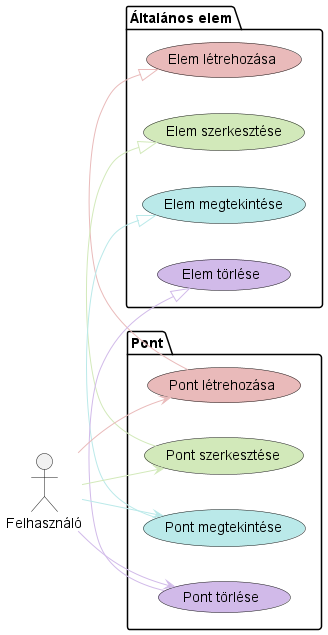
\includegraphics[width=0.30\textwidth, height=0.4\textheight]{figures/Point Diagram.png} & 
        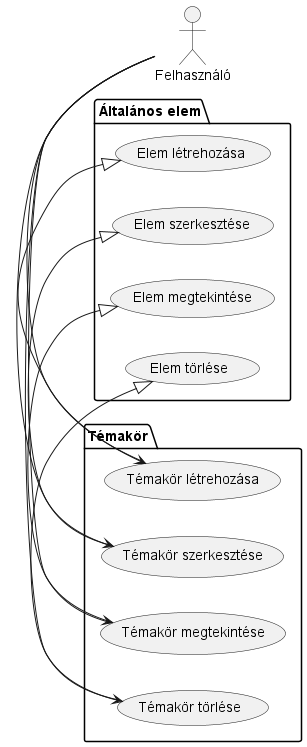
\includegraphics[width=0.30\textwidth, height=0.4\textheight]{figures/Topic Diagram.png} & 
        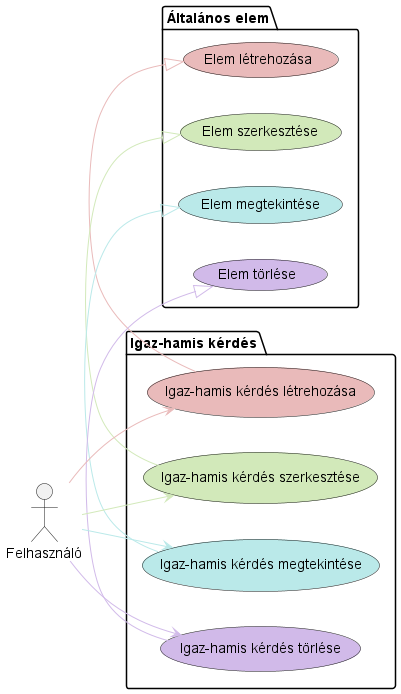
\includegraphics[width=0.30\textwidth, height=0.4\textheight]{figures/TrueFalseQuestion Diagram.png} \\
        
        % Második sor
        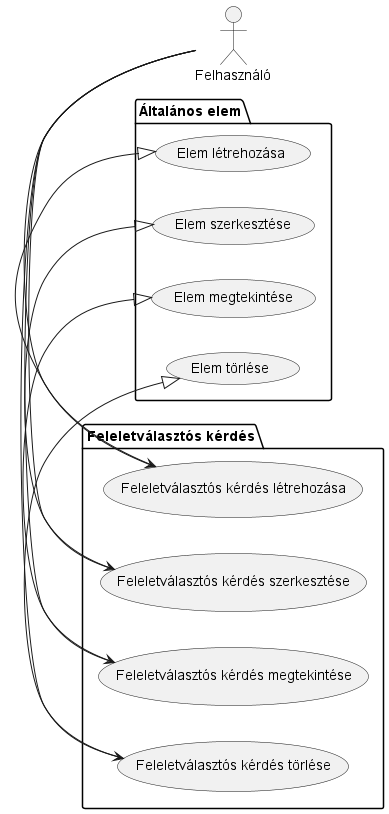
\includegraphics[width=0.30\textwidth, height=0.4\textheight]{figures/MultipleChoiceQuestion Diagram.png} & 
        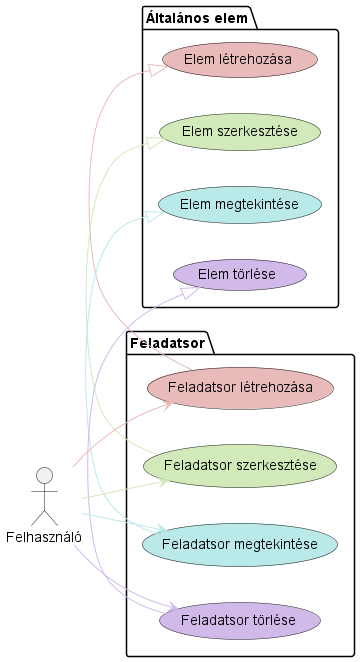
\includegraphics[width=0.30\textwidth, height=0.4\textheight]{figures/Exam Diagram.png} & 
        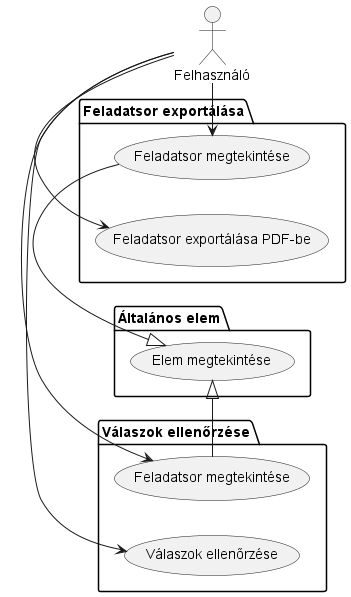
\includegraphics[width=0.30\textwidth, height=0.4\textheight]{figures/AnswerCheck Diagram.png}
    \end{tabular}
    \caption{Az alkalmazás használati eset diagramja.}
    \label{fig:UsecaseDiagram}
\end{figure}
